
\renewcommand{\arraystretch}{2}
\renewcommand{\figurename}{Figure}
\chapter{Literature Analysis and State of Art}
\label{chapter:literarure}

\newenvironment{literature}
{\quote\itshape}
{\endquote}

\begin{literature}
This chapter delves into the definition and categorization of weapons, while also elucidating the concept and significance of CCTV. Deep learning approaches and algorithms employed for this purpose are thoroughly analyzed. Additionally, the contributions of other authors in this field are dissected, offering a comprehensive review of their methodologies and findings. A significant portion of this chapter is dedicated to examining the datasets used by these scholars, highlighting their relevance, comprehensiveness, and potential limitations in the context of real-time weapon detection.
\end{literature}

\section{Context}
\subsection{Weapons}
The Cambridge Dictionary\footnote{https://dictionary.cambridge.org/dictionary/english/weapon} defines a weapon as "any object used in fighting or war, such as a gun, bomb, knife, etc.". This definition suggests that a weapon encompasses any tool or instrument intended to inflict damage or harm, whether on living beings, structures, or systems. Weapons have diverse applications, ranging from hunting and self-defense to warfare. However, their fundamental purpose remains unchanged: they amplify the user's ability to exert force, in either an offensive or defensive capacity.

Weapons can be categorized based on various criteria, including their range, mechanism, or intended use. However, this study will primarily focus on two categories: firearms and melee weapons.

Melee weapons are close-combat instruments that require the user to be in direct proximity to their target, like swords, daggers, maces, and clubs.

Firearms are a subset of ranged weapons that discharge projectiles powered by rapidly expanding high-pressure gas from chemical reactions. They can be further categorized into:
\begin{itemize}
    \item Handguns: Small, handheld firearms like pistols and revolvers.
    \item Rifles: Designed for accuracy, rifles have a longer barrel and are often used in situations requiring precision.
    \item Shotguns: These fire shells that contain multiple pellets, making them effective at close range.
    \item Automatic and Semi-Automatic: Automatic firearms continuously fire bullets as long as the trigger is pressed, while semi-automatics require a trigger pull for each shot.
\end{itemize}

\begin{figure}[h]
    \centering
    \begin{minipage}{0.45\textwidth}
        \centering
        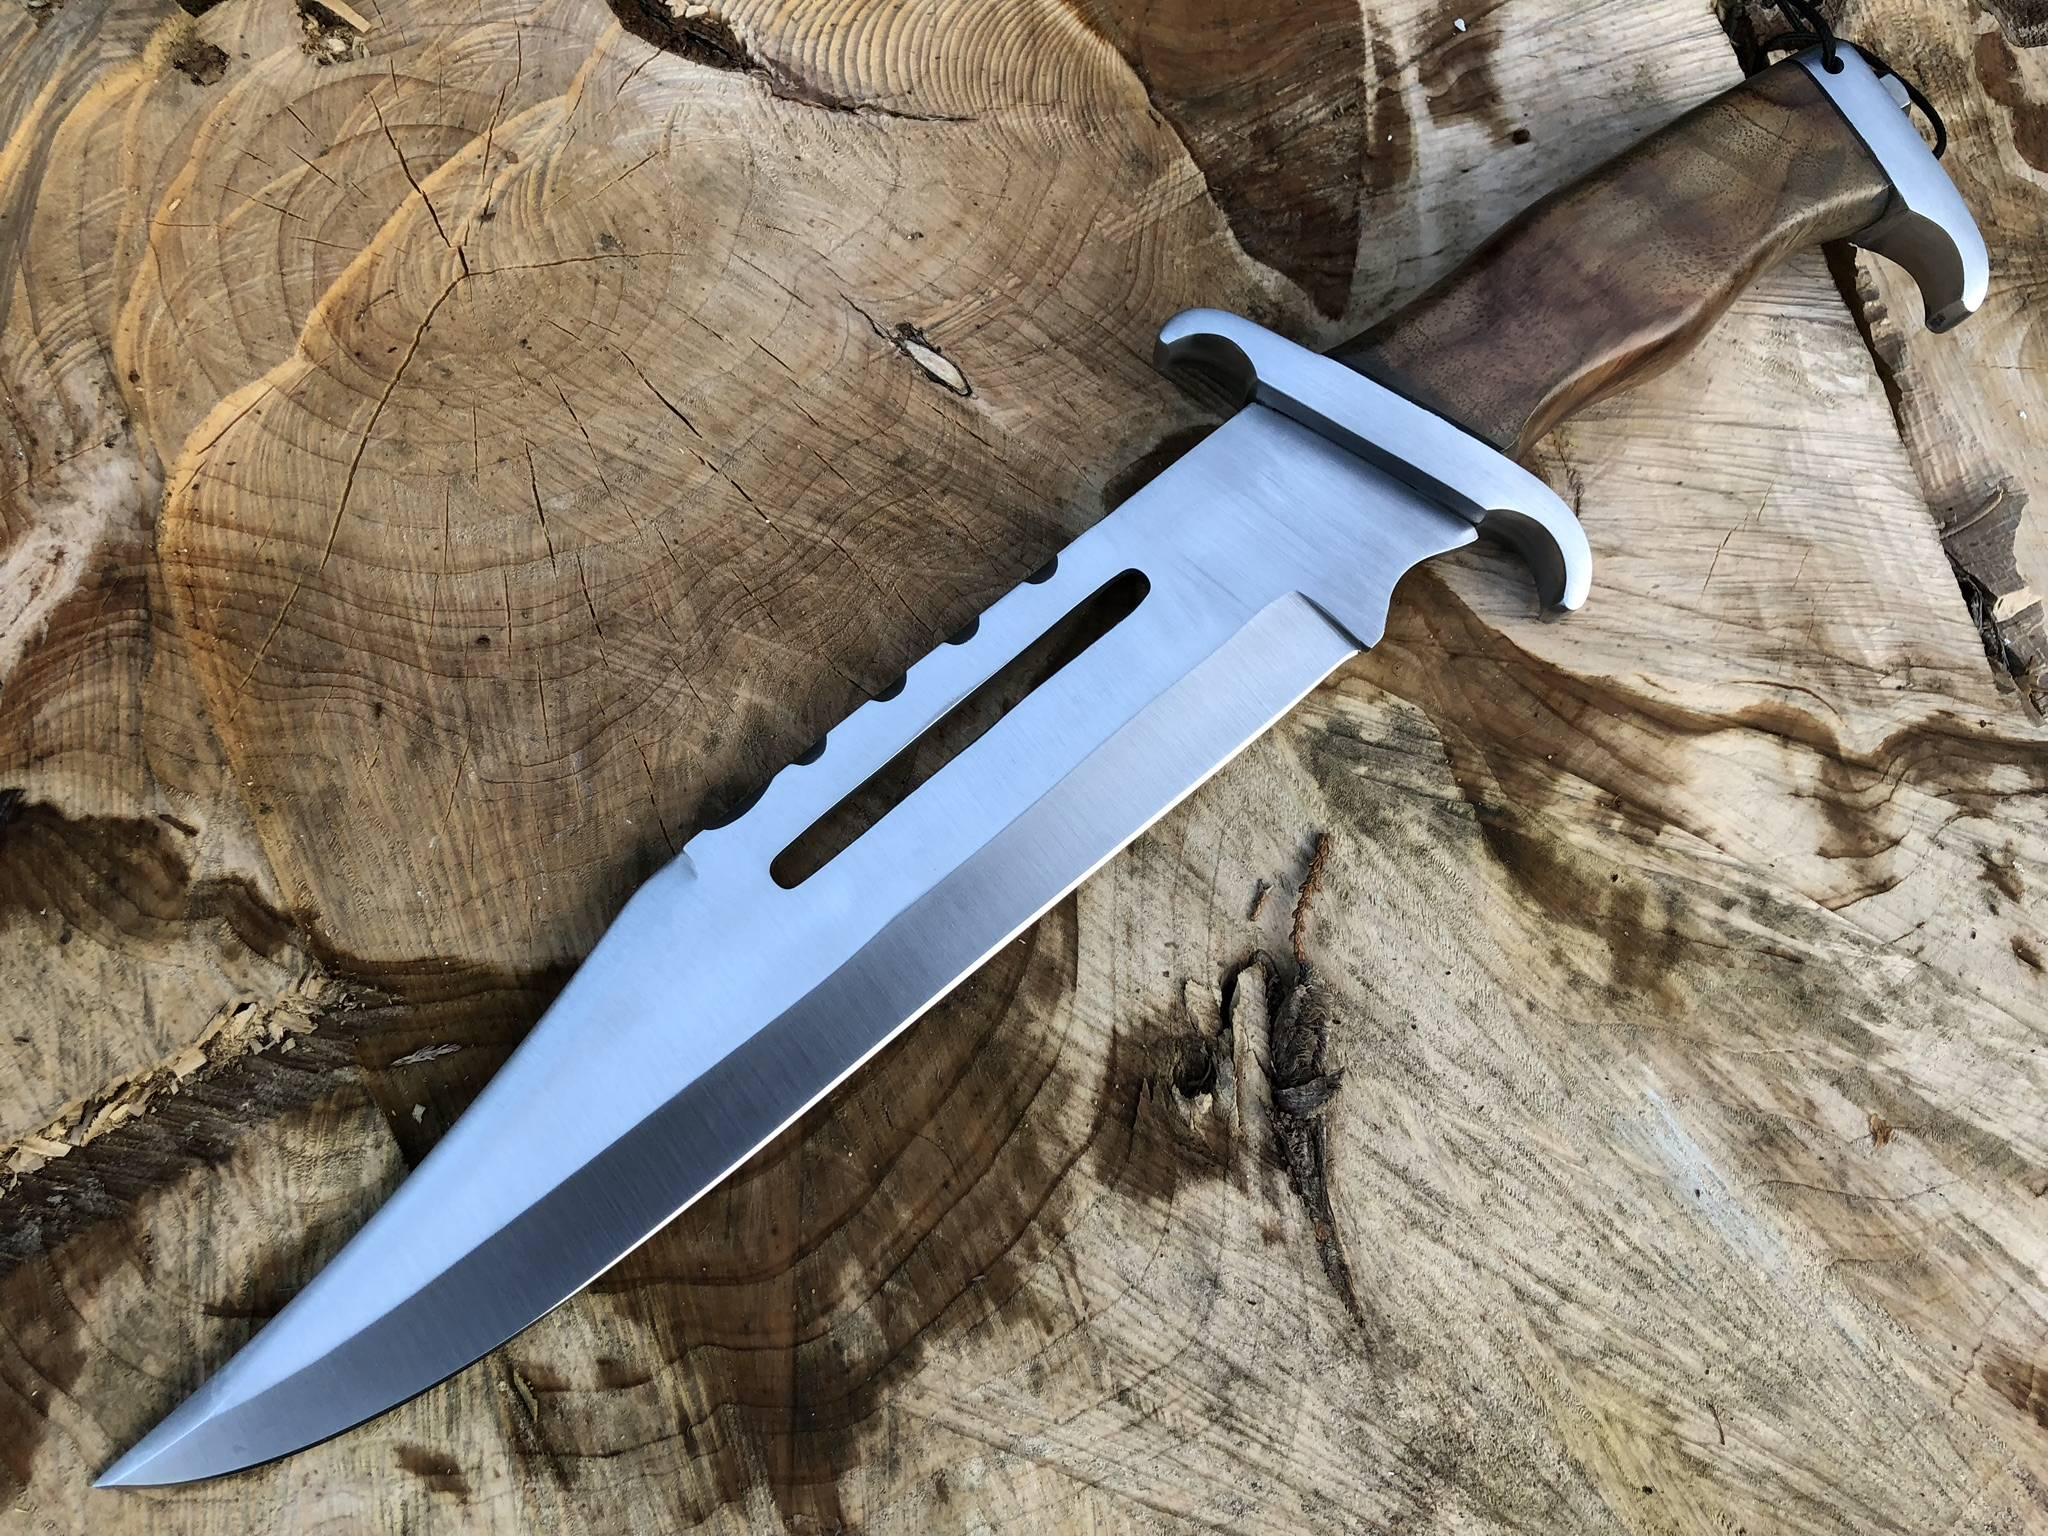
\includegraphics[width=1\linewidth]{figs/knife.jpg}
        \caption{Knife Example}
        \label{fig:first_image}
    \end{minipage}\hfill
    \begin{minipage}{0.48\textwidth}
        \centering
        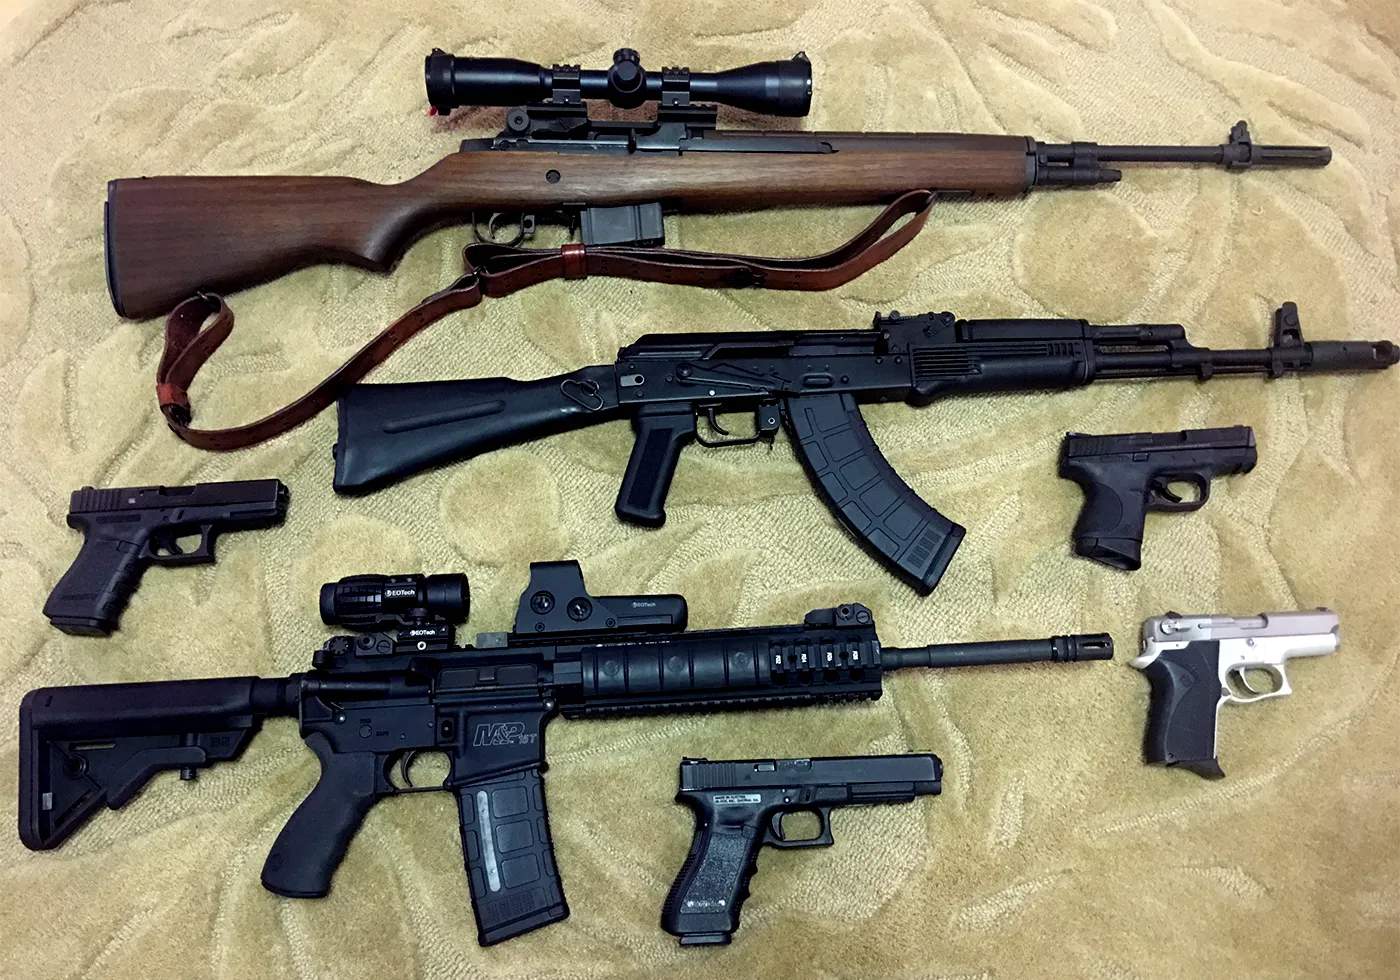
\includegraphics[width=1\linewidth]{figs/firearm.png}
        \caption{Different Firearms Example}
        \label{fig:second_image}
    \end{minipage}
\end{figure}

\subsection{\acl{cctv} (\ac{cctv})}
\ac{cctv} refers to a video surveillance system comprising strategically positioned cameras in various locations. These cameras capture footage, which is then transmitted to monitors for both real-time observation and later playback.

The primary goal of a \ac{cctv} system is to enhance area security through persistent surveillance of key areas. This is highly beneficial for large spaces or sites containing valuable or sensitive items. Besides recording, \ac{cctv} can issue alerts for detected motion, especially during off-hours in vacant business premises. These alerts are crucial for quickly informing authorities about possible security threats.

Additionally, \ac{cctv} systems are not only instrumental in monitoring activities during both operational and non-operational hours but also serve as crucial tools in identifying suspects in criminal activities.

\begin{figure}[h]
    \centering 
    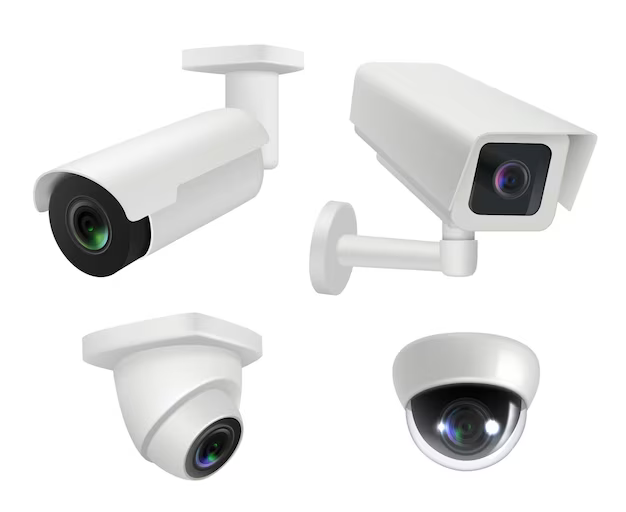
\includegraphics[width=0.35\textwidth]{figs/cctv.png} 
    \caption{\ac{cctv} Example}
    \label{fig:cctv}
\end{figure}

\section{Object Detection Overview}
\subsection{General Concepts in Object Detection}
Object detection stands as a vital component in the realm of computer vision. \selectlanguage{english}\citet{rfc2} describe its goal as "to determine where objects are located in a given image (object localization) and which category each object belongs to (object classification)", undertaking the dual challenge of not only locating an object within the visual frame, creating a bounding box around it, but also determining its category. \selectlanguage{english}\citet{rfc9} further reinforce this stating "Object detection is a fusion of object location and object classification task".

\begin{figure}[h]
    \centering 
    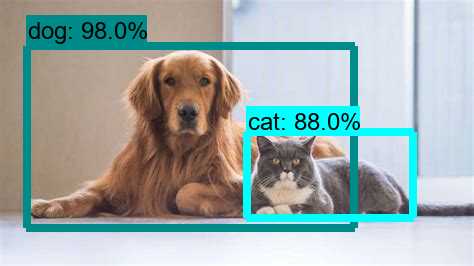
\includegraphics[width=0.5\textwidth]{figs/object-detection.png} 
    \caption{Object Detection Image ~\cite{rfc15}}
    \label{fig:object-detection}
\end{figure}

Object detection entails the identification of objects within images and videos. The process of recognizing these objects is fundamentally rooted in the training of object detection models. This crucial training phase involves several key steps:
\begin{itemize}
    \item \textbf{Data Collection}: Gathering a diverse set of images, each showcasing the object in a variety of contexts, including different backgrounds and angles.
    \item \textbf{Labeling}: Annotating each image with labels to show where the object is and confirming its presence
    \item \textbf{Feature Learning}: The neural network learns the object's unique features (like shape, color, texture, patterns) from these labeled images.
    \item \textbf{Generalization}: The ultimate goal of this training is to enable the neural network to not just recognize the object in the training images, but to generalize this knowledge. This allows the model to accurately identify and locate the object in new, unseen images.
\end{itemize} 

The 2014 milestone, \ref{fig:stage-detectors}, marks a pivotal before-and-after in AI applications \selectlanguage{english}\cite{rfc22}. Before, the field predominantly utilized traditional methods for tasks like object detection. These methods involved a multi-step process beginning with the selection of regions in images, which was often inefficient and computationally expensive due to the use of techniques like multi-scale sliding windows. Following this, feature extraction methods such as HOG, Haar-like, and SIFT were employed, but these struggled with variability in backgrounds and lighting conditions. The final step, classification, relied on algorithms like Adaboost, but these traditional techniques frequently fell short in terms of accuracy and efficiency \selectlanguage{english}\cite{rfc9}.

After 2014, the landscape of AI research underwent a significant transformation with the advent of deep learning-based methods. These new techniques, including Faster RCNN, SSD, and YOLO, revolutionized object detection by automatically learning feature representations from data. This shift not only addressed the limitations of the traditional methods, such as high computational costs and inadequate feature representation, but also led to substantial improvements in both the accuracy and efficiency of object detection processes.

\begin{figure}[h]
    \centering 
    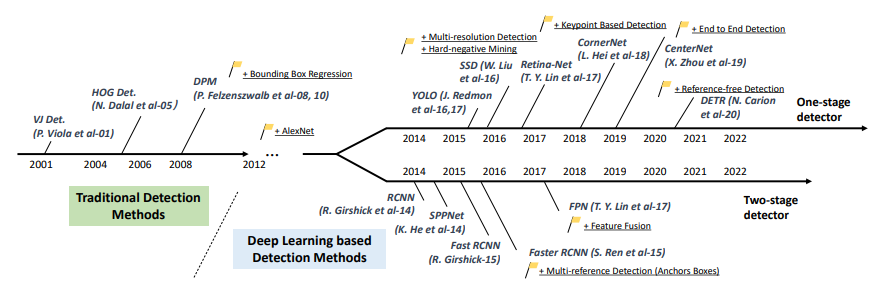
\includegraphics[width=0.9\textwidth]{figs/roadmap-stage.png} 
    \caption{Roadmap of object detection~\cite{rfc22}}
    \label{fig:stage-detectors}
\end{figure}

There are two primary methodologies, \ref{fig:stage-detectors}, employed for identifying and classifying objects. These methodologies differ significantly in their operational approach and performance characteristics.

Firstly, there is the \textbf{two-stage} detection process. This method involves an initial step of identifying potential areas of interest within the image. Subsequently, these identified regions undergo further analysis to classify the objects and refine their spatial boundaries. \selectlanguage{english}\cite{rfc21} emphasizes that while this approach is characterized by its high accuracy, it is generally slower in processing, a trade-off reflective of its intricate analytical process.

Conversely, the \textbf{single-stage} detection method simplifies the process by directly analyzing the image to determine object classifications and their spatial coordinates. As \selectlanguage{english}\cite{rfc21} points out, this method is much faster, providing a swift analysis of images. However, this speed comes at the cost of reduced accuracy compared to the two-stage approach.

Due to the variety of existing models and in order to understand which is the most appropriate, there are several metrics that allow determining and comparing the predictive performance of different object detection models. The two predominant metrics are Intersection over Union (IoU) and Average Precision (AP).

Intersection over Union~\cite{rfc14}, Figure \ref{fig:iou}, is a good metric to calculate localization accuracy and determine localization errors in object detection models. By dividing the intersection by the union, IoU offers the ratio of overlapping area to the entire area, thus effectively indicating the proximity of the predicted bounding box to the true bounding box.

Average Precision (AP)~\cite{rfc14} is determined by the area below the precision-recall curve for a set of predictions.

Recall represents the proportion of correctly identified instances out of all actual instances for a given class. On the other hand, precision is the proportion of true positives in relation to all the predictions made by the model.

Recall and precision offer a trade-off that is graphically represented into a curve by varying the classification threshold. The area under this curve produces the Average Precision for each class. Taking the mean of this metric across all classes results in the mean Average Precision (mAP).

\subsection{Object Detection Techniques Reviews}
This section explores the prevailing algorithms and techniques for object detection. To ensure a comprehensive overview, an extensive search was conducted across multiple online repositories and databases, sourcing both pioneering works and recent advancements to provide a balanced and in-depth perspective on the topic. To pursuit this objective, the selected reviews\footnote{comprehensive overview or evaluation of existing literature on a particular topic} are subsequently analyzed in greater detail, delving into their methodologies, findings, and implications for the field, offering a richer understanding of the evolution and current state of object detection techniques.

\selectlanguage{english}\citet{rfc2} delve into the evolution of detection methods, offering a comprehensive review of deep learning-based object detection frameworks. The review starts with a historical overview of deep learning, highlighting the role of CNN\footnote{Convolutional Neural Networks}. The focus then shifts to generic object detection architectures, discussing modifications and strategies to enhance detection performance. Through experimental analyses, various methods for detection tasks are compared, and insightful conclusions are drawn.

\selectlanguage{english}\citet{rfc8} embark on a journey through the intricate landscape of image processing techniques, presenting a meticulous review of machine learning-powered visual interpretation frameworks. Beginning with the rudiments of computational vision, the study underscores the pivotal role of array-based media computation in today's digital age. The discourse then transitions into a deep dive into prominent image processing algorithms like Single Shot Detection (SSD), Faster Region based Convolutional Neural Networks (Faster R-CNN), and You Only Look Once (YOLO). These algorithms are intricately dissected, revealing the architectural nuances, operational methodologies, and unique features that distinguish them from one another. Through systematic experimentation using datasets like Microsoft COCO, the researchers juxtapose these algorithms, offering profound insights into their individual strengths and caveats.

With their review, \selectlanguage{english}\citet{rfc9} underscore the nuances of computer vision, accentuating the transformative role of Deep Convolutional Neural Networks (DCNNs). Their study, while sweeping across various applications from video processing to speech recognition, zeroes in on object detection's pivotal role in fields like transportation and security. They also shed light on pivotal evaluation metrics, notably Average Precision (AP), essential for gauging detector effectiveness. Emphasizing the historical shift from traditional methods to deep learning post-2014, they meticulously dissect frameworks like SSD and YOLO. By juxtaposing these with older techniques and analyzing their performance on datasets like PASCAL VOC and MS COCO, the authors provide invaluable insights into the ever-evolving landscape of object detection.

\selectlanguage{english}\citet{rfc10} delve deep into the expansive realm of deep learning (DL), offering a comprehensive review of its concepts, convolutional neural network (CNN) architectures, challenges, applications, and prospective directions. The paper starts by highlighting the rising dominance of the DL paradigm, asserting its position as the "Gold Standard" in the machine learning community. Notably, the authors elucidate the unparalleled capability of DL to learn from massive datasets, outpacing traditional approaches in various applications. Venturing further, the discussion unfolds around pivotal CNN architectures, shedding light on their design intricacies and operational mechanisms. The challenges encountered in DL, be they computational or conceptual, are thoroughly explored. Additionally, the authors venture into the myriad of applications where DL has showcased exceptional performance, matching or even surpassing human capabilities.

\section{Related Work}
In the pursuit of a deeper understanding and improvement in weapon detection, numerous pivotal studies have emerged, highlighting various techniques, methodologies, and datasets. This section presents a thorough overview of these significant contributions, organizing the discussion into three core subsections: research methods, other author's articles, and datasets.

The initial part of the exploration dives into the research methods. This subsection details the approach taken to locate and identify pertinent literature. Given the vast amount of available works, a strategic filtration process was applied to select articles that are of paramount relevance to the topic of weapon detection.

Moving to the core of this section, a detailed examination of the articles\footnote{detailed written discourse on a specific subject} is undertaken. Each article is analyzed with respect to its primary objectives, methodologies, and outcomes. In an endeavor to furnish readers with a granular understanding, the techniques and architectures proposed by various scholars are further dissected.

Lastly, the focus shifts to the datasets\footnote{collection of related data points, often organized in tables, arrays, or other structures.}. This part furnishes a detailed overview of the datasets employed in weapon detection research. The narrative explores the origins of these datasets, the methods used for their sourcing, and underscores their distinguishing features.

\subsection{Research Method}
To initiate this study, a comprehensive review of existing research and projects in this field, with analogous objectives, was imperative. To facilitate this literature survey, the Scopus\footnote{\url{https://www.scopus.com/home.uri}} database, renowned for its vast collection of academic and research publications, was employed.

Due to the vast number of articles across diverse disciplines, it was necessary to make a careful selection. Consequently, specific keywords were utilized to pinpoint articles pertinent to the dissertation's subject matter.

So, utilizing Scopus, a search was executed with the query: ("deep" AND "learning" AND "real" AND "time" AND "weapon" AND "detection"). From the 70 records retrieved, a meticulous selection process resulted in 8 articles that align closely with the theme of this study, as illustrated in Figure \ref{fig:cctv}.

\begin{figure}[h]
    \centering 
    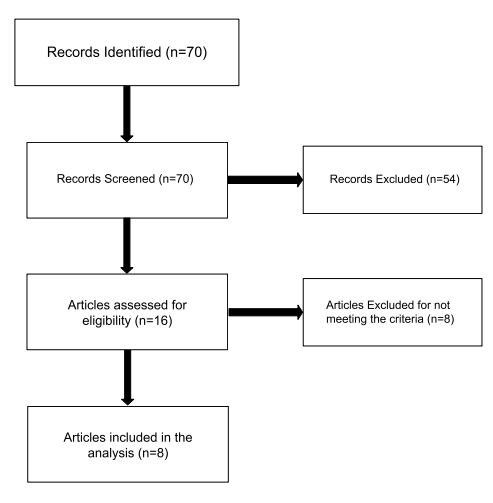
\includegraphics[width=0.37\textwidth]{figs/scopus.png} 
    \caption{Scopus Query, Author's own}
    \label{fig:scopus_query}
\end{figure}

\subsection{Articles}
\selectlanguage{english}\citet{rfc3} address the pressing concern of rising incidents involving firearms and knives due to insufficient security checks. Noting that while CCTVs have become prevalent, their constant surveillance demands often surpass human monitoring capabilities. The paper primarily introduces an automated weapon detection system, which employs the YOLOv5 deep learning model, tailored to a specially curated dataset. This innovation excels in the detection of various firearms and knives, showcasing an impressive F1 score of 0.95 when applied to CCTV footage. The study underscores the potential of neural networks and AI in enhancing real-time security measures.

In a world increasingly focused on security and safety, \selectlanguage{english}\citet{rfc4} emphasize the vital role of establishing a secure environment to bolster economic growth, especially for investors and tourists. While CCTV cameras have been a cornerstone for surveillance, their dependency on human monitoring highlights a gap in ensuring continuous vigilance. Recognizing the challenges of real-time weapon detection — such as varied viewing angles, occlusions, and carrier concealment — the research undertakes the task of leveraging advanced, open-source deep learning algorithms to detect potential threats. Given the absence of a standardized dataset, the researchers meticulously curated their own, drawing from diverse sources, including original photos, online repositories, and even film databases. Their exploration spanned several algorithms, like VGG16, Inception variants, and YOLO iterations. Through rigorous testing prioritizing precision and recall over mere accuracy, YOLOv4 emerged as the frontrunner, achieving a notable F1-score of 91\% and a mean average precision of 91.73\%, setting a new benchmark in the field.

In the research conducted by \selectlanguage{english}\citet{rfc5}, the growing menace of illicit firearms in public spaces despite the omnipresence of CCTVs is highlighted. While CCTVs offer visual insights, the human element in consistently monitoring vast streams of footage often leads to oversights, especially in detecting concealed weapons. Addressing this gap, the study introduces an advanced weapon detection methodology leveraging the YOLOv5 deep learning framework. This model is fine-tuned to a dataset comprising 1496 images and demonstrates a superior ability to detect handguns in varied scenarios. Notably, the system achieved an impressive mean average precision (mAP) of 91.76\% when tested. A comparative analysis, Figure \ref{fig:performance-Thangaraj}, with the YOLOv3 model revealed that YOLOv5 not only has enhanced accuracy in handgun detection but also offers faster detection speeds and is computationally less demanding.

\begin{figure}[h]
    \centering 
    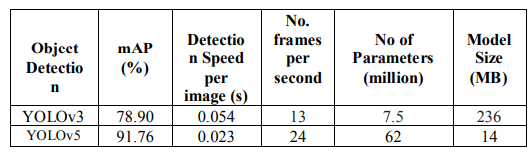
\includegraphics[width=0.55\textwidth]{figs/performance-Thangaraj.png} 
    \caption{\selectlanguage{english}\citet{rfc5} Models Performance Comparison}
    \label{fig:performance-Thangaraj}
\end{figure}

In the context of Smart Cities, \selectlanguage{english}\citet{rfc18} address the urgent need for enhanced urban security through advanced surveillance. While CCTVs are prevalent, the sheer volume of visual data often challenges human analysis. The authors present a novel approach, combining super-resolution techniques with the YOLOv4 deep neural network, to detect knives in complex images, a task made difficult by variables like shape, size, and lighting. Their research showcases the potential of AI surveillance to enhance real-time security, making video footage not just viewable but actionable and quantifiable. This study sets the stage for future extensions, such as firearm detection, and works as a testament to the transformative power of AI in urban safety protocols.

In the study by \selectlanguage{english}\citet{rfc17}, the escalating urban crime rates, particularly involving firearms and sharp objects, are brought to the forefront. While CCTVs are omnipresent in modern cities, the vast amount of data they produce often overwhelms manual surveillance efforts. Addressing this gap, the authors have developed a cutting-edge solution using the YOLOv8 deep learning framework, fine-tuned on a custom dataset comprising images of pistols, knives, and screwdrivers. The system, Figure \ref{fig:safa-architecture}, not only identifies weapons but also evaluates potential threat levels by analyzing the arm position of the person in possession. Demonstrating a notable 93\% accuracy on CCTV recordings, the study exemplifies the transformative role of AI in enhancing urban security protocols.

\begin{figure}[h]
    \centering 
    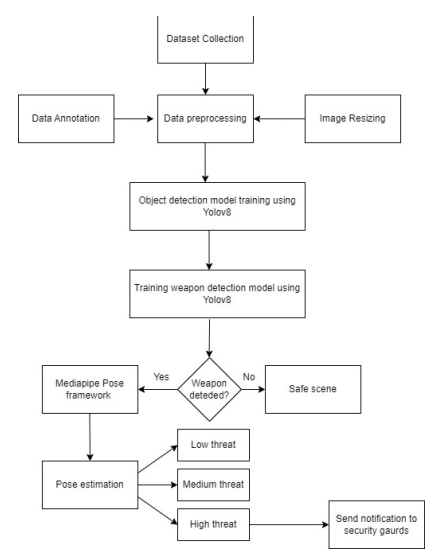
\includegraphics[width=0.55\textwidth]{figs/safa-architecture.png} 
    \caption{\selectlanguage{english}\citet{rfc17} Solution Architecture}
    \label{fig:safa-architecture}
\end{figure}


\selectlanguage{english}\citet{rfc6} research tackles the increasingly alarming scenario of weapon-related threats in crowded public spaces like banks, airports, and railway stations. Recognizing that while the deployment of CCTV cameras has seen a global surge, the sheer volume of footage can overwhelm human operators. This paper introduces a sophisticated weapon detection system, Figure \ref{fig:gawade-architecture},  that uses the power of deep learning, specifically through the use of Convolutional Neural Networks (CNN). Trained on a comprehensive dataset of 10014 images, the model adeptly identifies knives, small guns, and long guns, achieving an admirable accuracy rate of approximately 85\%.

\begin{figure}[h]
    \centering 
    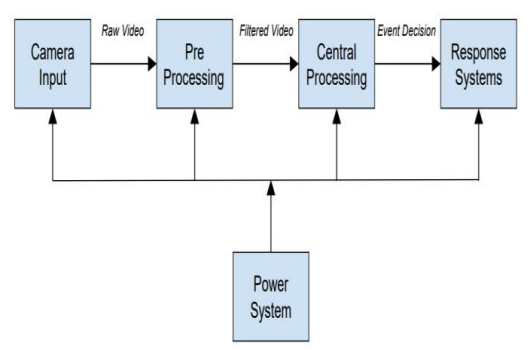
\includegraphics[width=0.55\textwidth]{figs/Gawade-architecture.png} 
    \caption{\selectlanguage{english}\citet{rfc6} Architecure Diagram}
    \label{fig:gawade-architecture}
\end{figure}

\selectlanguage{english}\citet{rfc19} introduce a forward-thinking security system architecture that uses deep learning and image-processing for real-time weapon detection in CCTV feeds. By periodically capturing images from these feeds and analyzing them using a convolutional neural network (CNN), the system can quickly identify potential threats. Upon detection, security personnel are promptly alerted via a mobile application, accompanied by an image of the potential threat. Impressively, the system claims a 92.5\% accuracy rate and can detect threats in a mere 1.6 seconds, underscoring the transformative potential of integrating AI with security protocols.

\selectlanguage{english}\citet{rfc20} highlight that while CCTV systems are everywhere, their efficacy is often hampered by the reliance on police personnel for monitoring. Addressing this challenge, the study introduces an integrated weapon detection system for CCTVs. Drawing from two public datasets, ARMAS and IMFDB, the research employs various object detection techniques, including SSD MobileNet-V1, EfficientDet-D0, and notably, Faster R-CNN Inception Resnet-V2. Specifically, the Faster R-CNN Inception V2, when used with the ARMAS dataset, achieved a mAP of 0.540, and Average Precision scores of 0.793 at 0.5 IoU and 0.627 at 0.75 IoU.

\selectlanguage{english}\citet{rfc7} emphasize the alarming rise in criminal activities in urban spaces, despite the ubiquity of CCTV systems in public areas. Recognizing the limitations of human supervision for these vast surveillance networks, they introduce an intelligent crime detection mechanism, Figure \ref{fig:shenoy-architecture}. Utilizing the SSD Mobilenet architecture fine-tuned on the DaSCI Weapon Dataset, their solution adeptly identifies a broad spectrum of weapons, yielding an accuracy rate of 81\%. Moreover, with the integration of the GRU-based behavior analysis model, the system achieved a notable accuracy of 95.97\% in detecting suspicious actions.

\begin{figure}[h]
    \centering 
    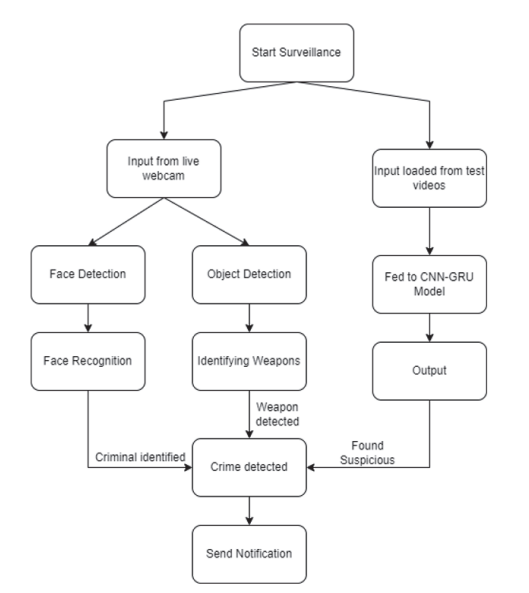
\includegraphics[width=0.55\textwidth]{figs/shenoy-architecture.png} 
    \caption{\citet{rfc7} System Architecture}
    \label{fig:shenoy-architecture}
\end{figure}

\subsection{Datasets}
In Rehman's study ~\cite{rfc3}, the dataset comprises three distinct classes: Short Guns, Long Guns, and Knives - Figure \ref{fig:rehman-dataset}. This dataset is gathered from a variety of platforms, including surveillance videos from YouTube, simulations of firearms and knives created within the Unity framework, and images of pistols, revolvers, and knives from the Open Images Dataset as well as Kaggle. For video sources, individual frames were extracted and subsequently labeled manually using the LabelImg Python utility. To enhance the model's training performance, data augmentation techniques were employed.

\begin{figure}[h]
    \centering 
    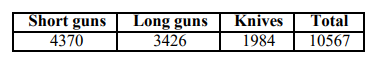
\includegraphics[width=0.45\textwidth]{figs/rheman-dataset.png} 
    \caption{\citet{rfc3} Dataset Images Classes Number}
    \label{fig:rehman-dataset}
\end{figure}

\selectlanguage{english}\citet{rfc4} focused on creating robust datasets for real-time weapon detection, specifically targeting the recognition of pistols within various environments. The data was meticulously gathered from diverse sources including the internet, YouTube CCTV videos, GitHub repositories, research groups, and the Internet Movie Firearm Database (imfdb.org).
They constructed three distinct datasets, being categorized into 'Pistol' and 'Not-Pistol' classes. The 'Pistol' class included pistols, revolvers, and other similar handheld weapons, while the 'Not-Pistol' class comprised objects often mistaken for weapons, such as wallets, cell phones, and metal detectors. This deliberate inclusion of 'confusion objects' in the 'Not-Pistol' class was a strategic approach to reduce false positives and negatives, thereby enhancing the precision and accuracy. For the data preparation and model training the researchers implemented data pre-processing steps to standardize the dataset, ensuring consistency in image size and resolution, and applied mean normalization. Also, used data augmentation strategies to artificially expand the dataset, improving the model's ability to generalize.

In the study conducted by \selectlanguage{english}\citet{rfc5}, models were trained using Google Collab, both Yolov3 and Yolov5, utilizing pre-trained weights on the COCO dataset ~\cite{rfc16}. The dataset, comprising 1496 images, was strategically segmented into training, validation, and testing sections. Out of these, 1200 images were allocated for training, while the remaining 296 were divided for both validation and testing, each one with 148. Training a model for 40 epochs took around 120 minutes, with a standard image size set at 416x416 pixels. Both YOLOv3 and YOLOv5 were trained within the PyTorch framework. The backbone feature extraction network, used across all experiments, was pre-trained using the COCO dataset. Additionally, fine-tuning of the backbone was allowed during training to enhance the representation of handguns.

\selectlanguage{english}\citet{rfc6} used a comprehensive dataset consisting of 10,014 distinct weapon images to train and evaluate the model's accuracy. These images were categorized into three primary object types: knives, with a total of 3,641 images; long guns, comprising 2,497 images; and small guns, which included 3,876 images. The dataset was strategically divided, allocating 80\% of the images (8,011 images) for training and the remaining 20\% (2,003 images) for testing. Each image used had a resolution of 240 x 240 pixels, and during the training phase, they were processed in batches of 32.

\selectlanguage{english}\citet{rfc7} employed two distinct datasets to train and evaluate the models. The first, the DaSCI Weapon Dataset, stands out in the realm of weapon detection for its ability to distinguish between weapons and commonplace objects. This dataset facilitated the training of the system to detect approximately 91 weapons of mass destruction. For the Suspicious Behavior Prediction module, the CAVIAR Dataset was utilized. This dataset comprises video clips representing six varied human actions. Annotations for these .mpg videos are stored in XML format, detailing both the role and context associated with each action. This information is crucial in determining whether a particular action can be classified as suspicious. To process this data, the XML file was parsed, aligning annotations with individual video frames. Each video was deconstructed frame by frame, extracting relevant data from the XML annotations. Subsequently, the data was labeled either as suspicious or not suspicious. 

\selectlanguage{english}\citet{rfc18} used two primary datasets to training and testing models related to knife detection in surveillance systems. The DaSCI Dataset focuses on knife detection, comprising 2,078 images with various visual features of knives. The images were mainly sourced from the internet, including YouTube videos. On the other hand, the MS COCO 2017 Dataset is a broader computer vision dataset with 330,000 images across 80 classes. Within this dataset, 4,326 images are labeled for the 'knife' class.

\selectlanguage{english}\citet{rfc17} faced challenges in gathering a comprehensive weapon dataset, particularly for knife and screwdriver images, due to the lack of labeled datasets suitable for classifier training. To address this, they employed web scraping techniques, sourcing images from various websites and GitHub repositories. Following the collection process, manual labeling of the images was undertaken using graphical annotation tools such as LabelImg and Roboflow. The images were then preprocessed to achieve a standardized resolution of 416 x 416. The final dataset comprised approximately 6,000 images: 2,000 each of pistols, knives, and screwdrivers. For model training and testing, the images were split in an 80:20 ratio, respectively.

\selectlanguage{english}\citet{rfc19} set up a Raspberry Pi B+ and camera 1.8m high, facing a lab entrance 4.5m away to capture images of consenting students entering and exiting. To simulate potential threats, students were provided with handgun replicas, with minimal guidance on how to hold them, resulting in a variety of poses. The dataset started with 14k images at 1920p x 1080 resolution. After data augmentation like scaling and rotation, it expanded to 28k images. A challenge was the gun's small size in images, increasing misclassification risks.

\selectlanguage{english}\citet{rfc20} sourced images of firearms-related crime intentions from two primary datasets: the ARMAS Weapon Detection Dataset, which contains 3,000 clear images of pistols, some held by individuals; and the IMFDB Weapon Detection System, which combines 4,940 diverse images of pistols and rifles from the Internet Movie Firearms Database and some CCTV footage. After collecting the data, the images were preprocessed to fit object detection training protocols and subsequently divided into training and testing subsets using an 80:20 ratio.

\section{Research Results}
\subsection{Weapon Detection Deep Learning Algorithms}
\subsection{Weapon Detection Datasets}